\documentclass[12pt, xcolor={usenames,dvipsnames,svgnames,x11names,table}]{beamer}

%%%%% make text revisible when compiled with XeLaTeX %%%%%
\makeatletter 
\def\beamer@framenotesbegin{% at beginning of slide
     \usebeamercolor[fg]{normal text}
     \gdef\beamer@noteitems{}% 
     \gdef\beamer@notes{}% 
}
\makeatother

%%%%% packages %%%%%
\usepackage{lipsum}					% für Testtexte
\usepackage{graphicx}				% für Bilder
\usepackage{geometry}				% für Seitenränder
\usepackage[utf8]{inputenc}			% für Zeichencodierung
\usepackage[T1]{fontenc}			% für Silbentrennung
\usepackage[english,ngerman]{babel}	% für Dokumentensprache
\usepackage{amsmath}				% für colle Mathesachen
\usepackage{amssymb}				% für colle Mathesachen
\usepackage{listings}				% für Programmiercode
\usepackage{tabularx}				% für bessere Tabellen
%\usepackage{subcaption}			% für Untertitel von Unterbildern
\usepackage{ulem}					% für Unterstreichungen usw.
%\usepackage{pifont}				% für tolle Symbole (Zapf Dingbats)
%\usepackage{enumerate}				% für bessere Aufzählungen
%\usepackage[section]{placeins}		% für Floats (setzt automatisch \FloatBarrier vor jeder neuen Section)
%\usepackage{tocloft}				% für Inhaltverzeichniseintrage ohne Nummerierung und Existenz im Text
\usepackage{pgfpages}				% für Dual-Screen-Präsentationen
\usepackage{hyperref}

%%%%% presentation template %%%%%
\setbeamertemplate{footline}[text line]{\parbox{\linewidth}{\vspace*{-8pt}Raumzeitliche Analyse von Twitter Daten\hfill\insertshortauthor\hfill\insertpagenumber}}
\setbeamertemplate{navigation symbols}{}

%%%%% presentation options %%%%%
%\setbeameroption{show notes on second screen = right}	% render note page to the right of frame
\hypersetup{pdfstartview={Fit}} 						% fits the presentation to the window when first displayed
\graphicspath{{pictures/}}								% picture path

%%%%% presentation theme %%%%%
\usetheme{Madrid}
\usecolortheme{default}


%%%%% presentation logo %%%%%
%\logo{\includegraphics[height=1.9cm]{picture}}

%%%%% presentation informations %%%%%
\title{Raumzeitliche Analyse von Twitter Daten}
\subtitle{Softwareentwicklungprojekt I}
\author{Niklas Baumbach, Felix Juch und Martin Immel}
\date{}

%%%%% listing style %%%%%
\lstdefinestyle{mystyle}{
	basicstyle = \scriptsize\ttfamily,
	breaklines = true,
	postbreak = \text{$\hookrightarrow$},
	numbers = left,
	numbersep = 10pt,
	numberstyle = \color{Gray},
	commentstyle = \color{DarkSlateGrey},
	stringstyle = \color{Purple},
	otherkeywords = {},
	keywords = [2]{},
	keywordstyle = {\color{Blue}},
	keywordstyle = [2]{\color{OliveGreen}},
	xleftmargin = .05\textwidth,
	literate={ä}{{\"a}}1 {ö}{{\"o}}1 {ü}{{\"u}}1 {ß}{{\ss}}1 {Ü}{{\"U}}1 {Ä}{{\"A}}1 {Ö}{{\"O}}1,
	escapeinside={[*}{*]}
}


%%%%% main %%%%%
\begin{document}
	\begin{frame}
	 	\titlepage
	\end{frame}	
	
	
	\section{Inhalt des Projekts}
	\begin{frame}{Inhalt des Projekts}{}
		\textbf{Ziele:}\\
		\begin{itemize}
			\item raumzeitliche Auswertung von Twitter-Daten zur Detektion und Analyse von Naturkatastrophen
			\item Clustern der geo-lokalisierten Tweets mit Krisenbezug 
			\item Implementierung eines geeigneten Clustering-Algorithmus $\rightarrow$ FDCA (\textit{Fast Density Clustering Algorithm})
			\item Erstellen eines Frameworks zum Test des Algorithmus und zur Simulation
		\end{itemize}
	\end{frame}
	
	
	\begin{frame}{Inhalt des Projekts}{Clustering}
	
		\textbf{FDCA-Clustering:}
		\\\bigskip
		\begin{columns}[c, onlytextwidth]
			\begin{column}{.45\textwidth}
				Dichte $\rho$ und Grenzdistanz dc:\\
				\bigskip
				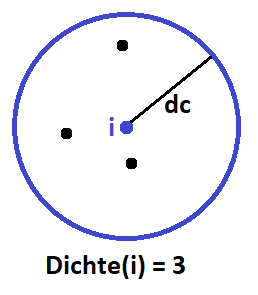
\includegraphics[scale=.9]{dc_dichte}
			\end{column}
			
			\begin{column}{.55\textwidth}
				\begin{itemize}
					\item dc = Grenzdistanz
					\item $\rho$ = Anzahl Datenpunkte in Grenzdistanz
				\end{itemize}
			\end{column}
		\end{columns}
		
	\end{frame}
	
	\begin{frame}{Inhalt des Projekts}{Clustering}
	
		\textbf{FDCA-Clustering:}
		\\\bigskip
		\begin{columns}[c, onlytextwidth]
			\begin{column}{.6\textwidth}
				Delta $\delta$:\\
				\bigskip
				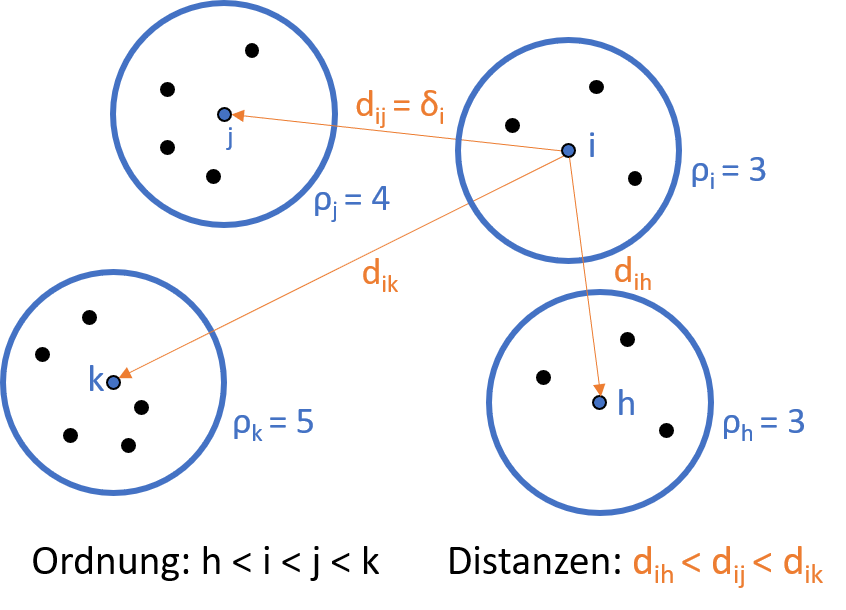
\includegraphics[scale=0.5]{delta}
			\end{column}
			
			\begin{column}{.4\textwidth}
				\begin{itemize}
					\item $\delta$ = minimaler Abstand zu Punkt höherer Dichte\\
					(bei gleicher Dichte: höhere Ordnung)
					\item Ordnung durch Index
				\end{itemize}
			\end{column}
		\end{columns}
		
	\end{frame}
	
	\begin{frame}{Inhalt des Projekts}{Clustering}
	
		\textbf{FDCA-Clustering:}
		\\\bigskip
		Clusterzentren bestimmen:\\
		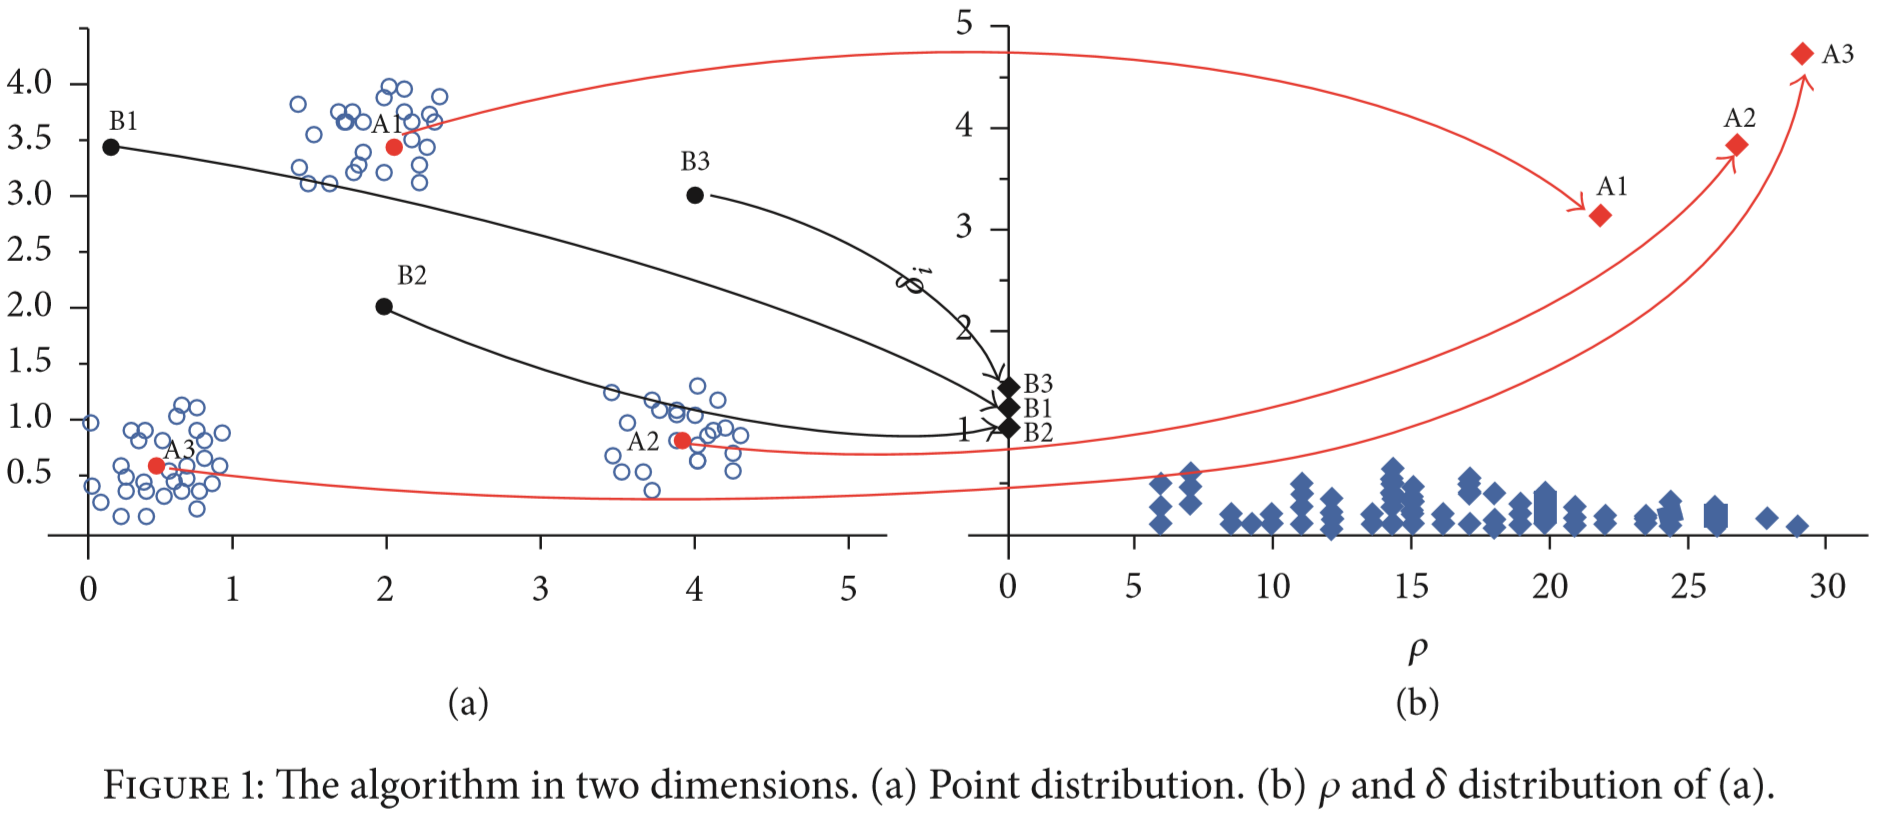
\includegraphics[scale=0.355]{rho_delta}
		
	\end{frame}
	
	\begin{frame}{Inhalt des Projekts}{Clustering}
	
		\textbf{FDCA-Clustering:}
		\\\bigskip
		Zuweisung der Cluster:
		\\\bigskip
		\center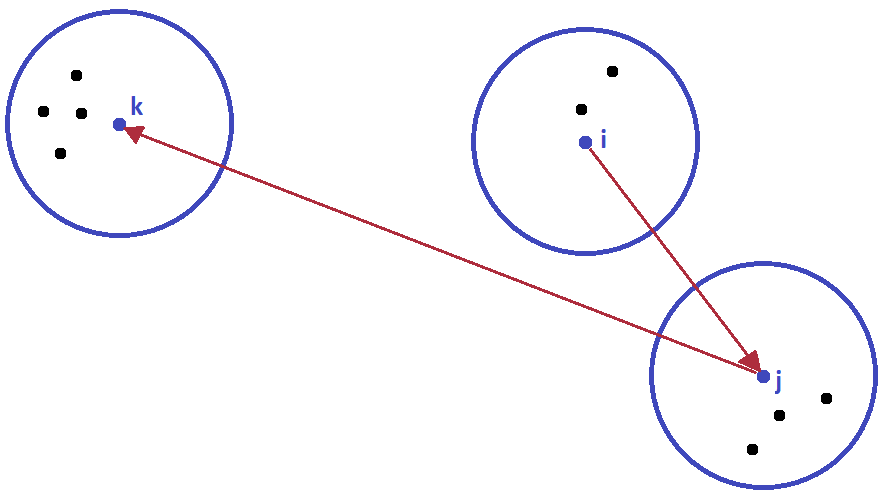
\includegraphics[scale=.6]{cluster_zuweisung}
		
	\end{frame}
	
	\section{Stakeholder}
	\begin{frame}{Stakeholder}{}
		\begin{columns}
			\begin{column}{.5\textwidth}
				\center 
\includegraphics[width=.9\textwidth]{dlr}
			\end{column}
			\begin{column}{.5\textwidth}
				\center 
\includegraphics[width=.8\textwidth]{fsu}
			\end{column}
		\end{columns}\bigskip
		\textbf{Betreuer:} Jens Kersten und Friedericke Klan
	\end{frame}
	
	
	% Überblick über das finale Ergebnis
	\section{}
	
	% Investierte Zeit pro Woche
	% Herausstellen der wesentlichen Leistungen
	\section{}
	

	% Überblick über nicht erreichte Ziele
	\section{}
	
	
	% ggf. Präsentation des Systems
	\section{}	
	
	\section{}
	\begin{frame}{Noch Fragen?}
		
\includegraphics[width=\textwidth]{fragen}
	\end{frame}
\end{document}

%%%%% empty frame with notes %%%%%

%	\begin{frame}{}{}
%		\note{
%			\begin{itemize}
%				\item
%			\end{itemize}
%		}
%		
%		
%	\end{frame}